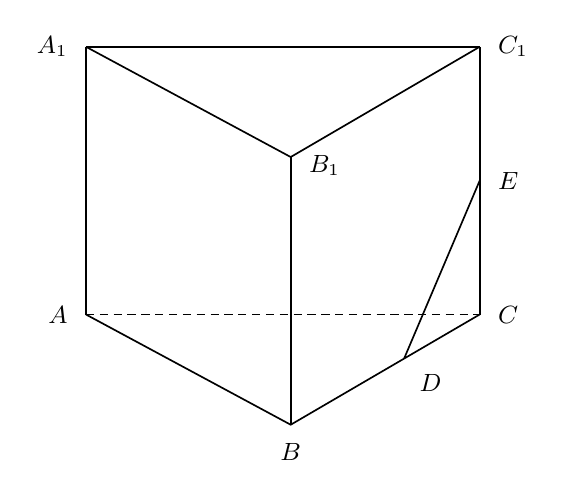
\begin{tikzpicture}[line width=0.6pt, font=\small]
\coordinate (A) at (0,0);
\coordinate (B) at (2.6,-1.4);
\coordinate (C) at (5.0,0);
\coordinate (A1) at (0,3.4);
\coordinate (B1) at (2.6,2.0);
\coordinate (C1) at (5.0,3.4);
\coordinate (D) at (4.0400000000,-0.5600000000);
\coordinate (E) at (5.0,1.7);
% top and verticals
\draw (A1) -- (C1);
\draw (A1) -- (A);
\draw (B1) -- (B);
\draw (C1) -- (C);
\draw (A1) -- (B1);
\draw (C1) -- (B1);
% bottom: A-C dashed, A-B and B-C solid (D on BC)
\draw[densely dashed] (A) -- (C);
\draw (A) -- (B) -- (C);
% D-E segment
\draw (D) -- (E);
\node[left=3pt] at (A1) {$A_{1}$};
\node[right=3pt] at (C1) {$C_{1}$};
\node[right=2pt,xshift=1pt,yshift=-3pt] at (B1) {$B_{1}$};
\node[left=3pt] at (A) {$A$};
\node[below=3pt] at (B) {$B$};
\node[right=3pt] at (C) {$C$};
\node[below right=2pt] at (D) {$D$};
\node[right=3pt] at (E) {$E$};
\end{tikzpicture}
